\documentclass{article}
\usepackage{tikz}
\usetikzlibrary{arrows,quotes,intersections,calc,angles,arrows.meta,graphs,backgrounds,shapes.misc,trees}
\begin{document}
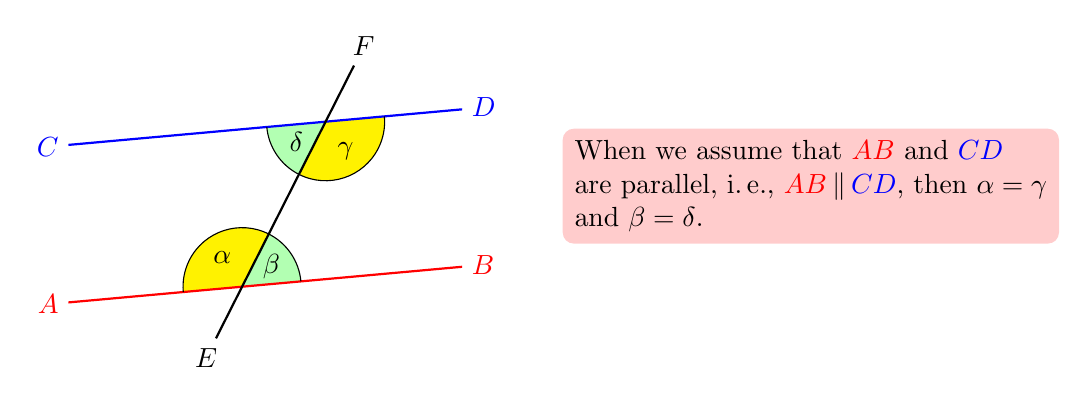
\begin{tikzpicture}[angle radius=.75cm]
\node (A) at (-2,0) [red,left] {$A$};
\node (B) at ( 3,.5) [red,right] {$B$};
\node (C) at (-2,2) [blue,left] {$C$};
\node (D) at ( 3,2.5) [blue,right] {$D$};
\node (E) at (60:-5mm) [below] {$E$};
\node (F) at (60:3.5cm) [above] {$F$};
\coordinate (X) at (intersection cs:first line={(A)--(B)}, second line={(E)--(F)});
\coordinate (Y) at (intersection cs:first line={(C)--(D)}, second line={(E)--(F)});
\path
(A) edge [red, thick] (B)
(C) edge [blue, thick] (D)
(E) edge [thick] (F)
pic ["$\alpha$", draw, fill=yellow] {angle = F--X--A}
pic ["$\beta$", draw, fill=green!30] {angle = B--X--F}
pic ["$\gamma$", draw, fill=yellow] {angle = E--Y--D}
pic ["$\delta$", draw, fill=green!30] {angle = C--Y--E};
\node at ($ (D)!.5!(B) $) [right=1cm,text width=6cm,rounded corners,fill=red!20,inner sep=1ex]
{
When we assume that $\color{red}AB$ and $\color{blue}CD$ are
parallel, i.\,e., ${\color{red}AB} \mathbin{\|} \color{blue}CD$,
then $\alpha = \gamma$ and $\beta = \delta$.
};
\end{tikzpicture}

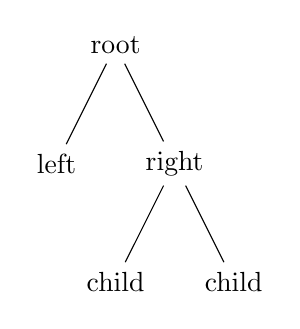
\begin{tikzpicture}
\node {root}
child {node {left}}
child {node {right}
child {node {child}}
child {node {child}}
};
\end{tikzpicture}

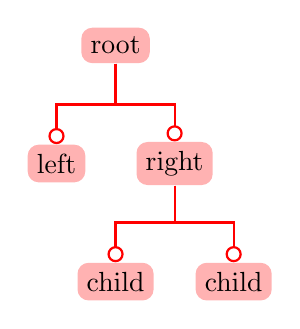
\begin{tikzpicture}
[edge from parent fork down, sibling distance=15mm, level distance=15mm,
    every node/.style={fill=red!30,rounded corners},
    edge from parent/.style={red,-o,thick,draw}]
    \node {root}
    child {node {left}}
    child {node {right}
    child {node {child}}
    child {node {child}}
    };
\end{tikzpicture}

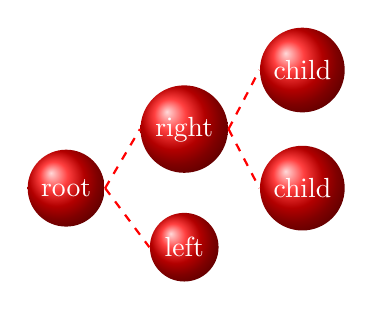
\begin{tikzpicture}
[parent anchor=east,child anchor=west,grow=east,
sibling distance=15mm, level distance=15mm,
every node/.style={ball color=red,circle,text=white},
edge from parent/.style={draw,dashed,thick,red}]
\node {root}
child {node {left}}
child {node {right}
child {node {child}}
child {node {child}}
};
\end{tikzpicture}

\tikz \graph [grow down, branch right] {
root -> { left, right -> {child, child} }
};

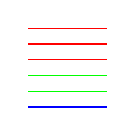
\begin{tikzpicture}
\begin{scope}[color=red]
\draw (0mm,10mm) -- (10mm,10mm);
\draw (0mm, 8mm) -- (10mm, 8mm);
\draw (0mm, 6mm) -- (10mm, 6mm);
\end{scope}
\begin{scope}[color=green]
\draw (0mm, 4mm) -- (10mm, 4mm);
\draw (0mm, 2mm) -- (10mm, 2mm);
\draw[color=blue] (0mm, 0mm) -- (10mm, 0mm);
\end{scope}
\end{tikzpicture}

 $A \mathbin{\tikz[baseline] \draw[->>] (0pt,.5ex) -- (3ex,.5ex);} B$
 
 Hello
\tikz[baseline=(X.base)]
\node [cross out,draw] (X) {world.};

Top align:
\tikz[baseline=(current bounding box.north)]
\draw (0,0) rectangle (1cm,1ex);

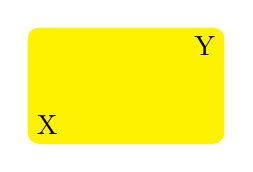
\begin{tikzpicture}[execute at end picture=%
{
\begin{pgfonlayer}{background}
\path[fill=yellow,rounded corners]
(current bounding box.south west) rectangle
(current bounding box.north east);
\end{pgfonlayer}
}]
\node at (0,0) {X};
\node at (2,1) {Y};
\end{tikzpicture}

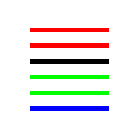
\begin{tikzpicture}[ultra thick]
\begin{scope}[red]
\draw (0mm,10mm) -- (10mm,10mm);
\draw (0mm,8mm) -- (10mm,8mm);
\end{scope}
\draw (0mm,6mm) -- (10mm,6mm);
\begin{scope}[green]
\draw (0mm,4mm) -- (10mm,4mm);
\draw (0mm,2mm) -- (10mm,2mm);
\draw[blue] (0mm,0mm) -- (10mm,0mm);
\end{scope}
\end{tikzpicture}
\end{document}